%==============================================================================
% Figure: Framework Venn Diagram
% Purpose: Show overlap and distinctions between Aether, Genesis, Pais
% Chapter: Ch17 - Framework Comparison
% Type: Conceptual
%==============================================================================

\begin{figure}[htbp]
  \centering
  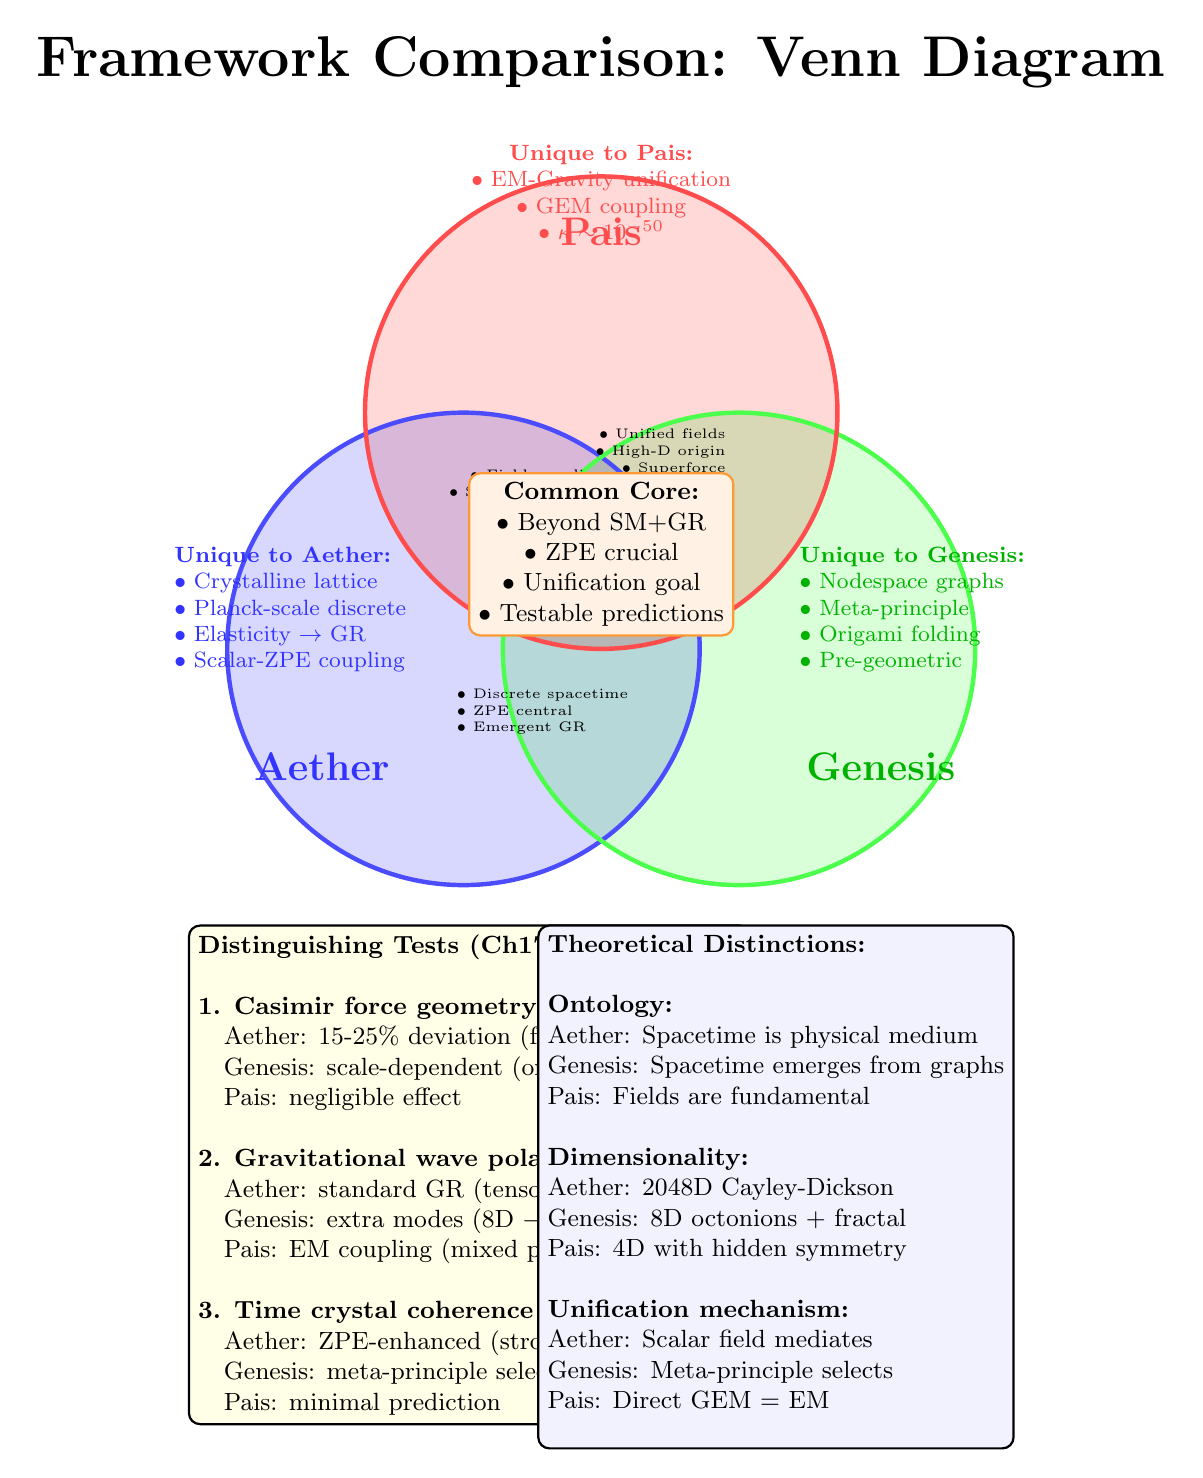
\begin{tikzpicture}[
    scale=1.0
  ]

    % Define circle styles
    \def\circleA{(0, 0) circle (3cm)}
    \def\circleG{(3.5, 0) circle (3cm)}
    \def\circleP{(1.75, 3) circle (3cm)}

    % Draw circles with transparency
    \begin{scope}[blend mode=multiply]
      \fill[blue!30, opacity=0.5] \circleA;
      \fill[green!30, opacity=0.5] \circleG;
      \fill[red!30, opacity=0.5] \circleP;
    \end{scope}

    % Draw circle outlines
    \draw[ultra thick, blue!70] \circleA;
    \draw[ultra thick, green!70] \circleG;
    \draw[ultra thick, red!70] \circleP;

    % Labels for each framework
    \node[font=\Large\bfseries, text=blue!80] at (-1.8, -1.5) {Aether};
    \node[font=\Large\bfseries, text=green!70!black] at (5.3, -1.5) {Genesis};
    \node[font=\Large\bfseries, text=red!70] at (1.75, 5.3) {Pais};

    % Unique features (non-overlapping regions)
    \node[font=\footnotesize, text=blue!80, align=left] at (-2.2, 0.5) {
      \textbf{Unique to Aether:} \\
      $\bullet$ Crystalline lattice \\
      $\bullet$ Planck-scale discrete \\
      $\bullet$ Elasticity $\to$ GR \\
      $\bullet$ Scalar-ZPE coupling
    };

    \node[font=\footnotesize, text=green!70!black, align=left] at (5.7, 0.5) {
      \textbf{Unique to Genesis:} \\
      $\bullet$ Nodespace graphs \\
      $\bullet$ Meta-principle \\
      $\bullet$ Origami folding \\
      $\bullet$ Pre-geometric
    };

    \node[font=\footnotesize, text=red!70, align=center] at (1.75, 5.8) {
      \textbf{Unique to Pais:} \\
      $\bullet$ EM-Gravity unification \\
      $\bullet$ GEM coupling \\
      $\bullet$ $\kappa \sim 10^{-50}$
    };

    % Pairwise overlaps
    % Aether + Genesis
    \node[font=\tiny, align=left, text=black] at (1.0, -0.8) {
      $\bullet$ Discrete spacetime \\
      $\bullet$ ZPE central \\
      $\bullet$ Emergent GR
    };

    % Genesis + Pais
    \node[font=\tiny, align=right, text=black] at (2.5, 2.5) {
      $\bullet$ Unified fields \\
      $\bullet$ High-D origin \\
      $\bullet$ Superforce
    };

    % Aether + Pais
    \node[font=\tiny, align=right, text=black] at (0.8, 2.0) {
      $\bullet$ Field coupling \\
      $\bullet$ Scalar mediation \\
      $\bullet$ 4D effective
    };

    % Central overlap (all three)
    \node[font=\small, align=center, text=black, draw=orange!80, fill=orange!10, rounded corners, thick]
      at (1.75, 1.2) {
      \textbf{Common Core:} \\
      $\bullet$ Beyond SM+GR \\
      $\bullet$ ZPE crucial \\
      $\bullet$ Unification goal \\
      $\bullet$ Testable predictions
    };

    % Experimental distinguishing tests (outside all circles)
    \node[anchor=north west, align=left, font=\small, draw=black, fill=yellow!10, rounded corners, thick]
      at (-3.5, -3.5) {
      \textbf{Distinguishing Tests (Ch17, Ch22):} \\
      \\
      \textbf{1. Casimir force geometry dependence} \\
      \quad Aether: 15-25\% deviation (fractal boundaries) \\
      \quad Genesis: scale-dependent (origami unfolds) \\
      \quad Pais: negligible effect \\
      \\
      \textbf{2. Gravitational wave polarization} \\
      \quad Aether: standard GR (tensor only) \\
      \quad Genesis: extra modes (8D $\to$ 4D) \\
      \quad Pais: EM coupling (mixed polarization) \\
      \\
      \textbf{3. Time crystal coherence} \\
      \quad Aether: ZPE-enhanced (strong effect) \\
      \quad Genesis: meta-principle selection \\
      \quad Pais: minimal prediction
    };

    \node[anchor=north east, align=left, font=\small, draw=black, fill=blue!5, rounded corners, thick]
      at (7.0, -3.5) {
      \textbf{Theoretical Distinctions:} \\
      \\
      \textbf{Ontology:} \\
      Aether: Spacetime is physical medium \\
      Genesis: Spacetime emerges from graphs \\
      Pais: Fields are fundamental \\
      \\
      \textbf{Dimensionality:} \\
      Aether: 2048D Cayley-Dickson \\
      Genesis: 8D octonions + fractal \\
      Pais: 4D with hidden symmetry \\
      \\
      \textbf{Unification mechanism:} \\
      Aether: Scalar field mediates \\
      Genesis: Meta-principle selects \\
      Pais: Direct GEM = EM \\
    };

    % Title
    \node[anchor=south, font=\huge\bfseries] at (1.75, 7.0) {Framework Comparison: Venn Diagram};

  \end{tikzpicture}
  \caption{Venn diagram comparing the Aether (blue), Genesis (green), and Pais (red) frameworks.
    The non-overlapping regions show unique features: Aether's crystalline lattice at Planck scale,
    Genesis's nodespace graphs and meta-principle, Pais's electromagnetic-gravity unification with
    coupling $\kappa \sim 10^{-50}$. Pairwise overlaps highlight shared concepts: Aether and Genesis
    both employ discrete spacetime with emergent general relativity; Genesis and Pais both invoke
    unified superforce concepts from higher dimensions; Aether and Pais both rely on field coupling
    mechanisms in effective 4D. The central orange region represents the common core: all three go
    beyond the Standard Model and General Relativity, treat zero-point energy as crucial, aim for
    unification, and make testable experimental predictions. The lower panels list distinguishing
    experimental tests (Ch22): Casimir force geometry dependence (Aether predicts 15-25\% deviation
    with fractal boundaries, Genesis shows scale-dependent effects, Pais minimal), gravitational
    wave polarization (extra modes for Genesis, EM coupling for Pais), and time crystal coherence
    (enhanced by ZPE in Aether). Theoretical distinctions include ontology (physical medium vs
    emergent graphs vs fundamental fields), dimensionality (2048D vs 8D+fractal vs 4D), and
    unification mechanisms (scalar mediation vs meta-principle vs direct GEM=EM).}
  \label{fig:framework-venn-diagram}
\end{figure}
